% Revision-5 presentation of the same complete independently audited 162,000 responses.
\begin{figure*}[t]
\centering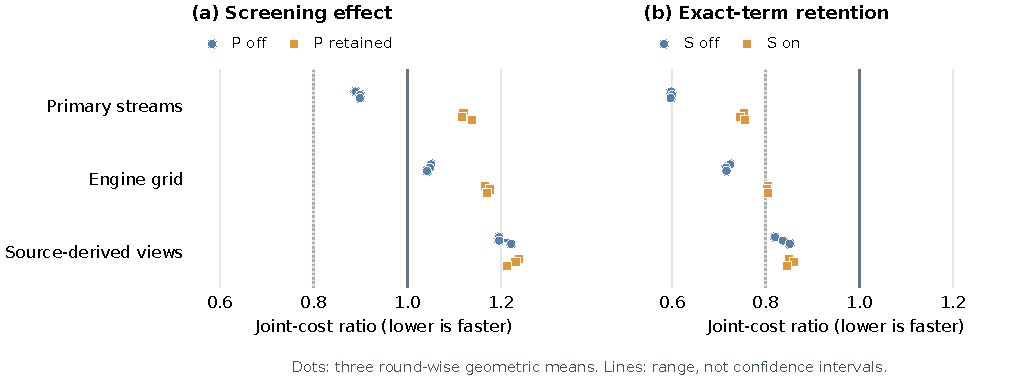
\includegraphics[width=\textwidth]{figures/checking_schedule_v4.pdf}
\caption{Isolating checking costs while preserving the same evidence and solver paths. Each dot is one timing round's equal-weight geometric-mean joint-cost ratio over all inputs in that group; the line shows its three-round range. Screening is compared at each fixed exact-term retention setting, and retention at each fixed screening setting. The $.8$ reference applies to the two registered primary contrasts only. Values below one indicate less total producer-and-receiver work; no interval is a statistical confidence interval.}
\label{fig:checking-factors}
\end{figure*}
\begin{table*}[t]
\centering\small
\caption{All registered factor and bridge comparisons. Entries are median [minimum, maximum] of the three round-wise geometric-mean joint-cost ratios. Original Prepared is lower-only and cannot prove false; Auto changes the simplex strategy. Their cost ratios are descriptive. Source-derived serving starts from saved views, excluding source ingestion.}
\label{tab:checking-factors}\begin{tabular}{lrrr}
\toprule
Contrast & Primary & Engine & Source-derived \\
\midrule
Screening, $P=0$ & 0.899 [0.889, 0.899] & 1.048 [1.042, 1.051] & 1.196 [1.196, 1.222] \\
Screening, $P=1$ & 1.120 [1.118, 1.138] & 1.170 [1.167, 1.177] & 1.231 [1.213, 1.238] \\
Exact retention, $S=0$ & 0.598 [0.597, 0.600] & 0.717 [0.715, 0.724] & 0.837 [0.820, 0.852] \\
Exact retention, $S=1$ & 0.753 [0.746, 0.756] & 0.804 [0.804, 0.805] & 0.849 [0.845, 0.862] \\
Both / original Prepared & 1.449 [1.449, 1.455] & 0.909 [0.899, 0.912] & 1.198 [1.184, 1.199] \\
Both / Auto bridge & 0.996 [0.959, 0.997] & 0.995 [0.994, 0.997] & 0.992 [0.990, 0.997] \\
\bottomrule
\end{tabular}

\end{table*}


All 1,134 plan-streams and 162,000 responses complete, with independent numerical replay and complete source bindings. The four core plans return identical evidence, decisions, routes and native-solver paths. Figure~\ref{fig:checking-factors} therefore isolates checking work rather than a change in which queries get answered. On the primary streams, screening with retained terms has round-wise ratios $1.120$, $1.118$, $1.138$; retaining exact terms with screening has ratios $0.753$, $0.746$, $0.756$. The joint requirement that both factors meet the registered primary engineering target is not supported. Table~\ref{tab:checking-factors} retains all six contrasts and both broader groups. The artifact includes every per-input ratio, prefix, factor interaction and decision comparison, including slow inputs and bridge losses. These are fixed-workload timing observations, not a significance or deployment-generalization claim.

\textbf{Caching changes whether screening pays.} Without retained exact terms, screening has primary ratios $0.889$--$0.899$; after retention, the same screening loses (Fig.~\ref{fig:checking-factors}). Retention without screening gives ratios $0.597$--$0.600$. Across the three primary inputs in each round, screening reduces exact dual checks from 6000 to 3003. With retained terms it saves 11.04--11.41\,s of producer verification, but screening itself costs 17.93--18.35\,s. These component timers explain the observed tradeoff; they are not added again to joint cost. A filter that avoids checks can therefore become uneconomic after those checks have been made cheaper. The broader groups also lose from screening under both retention settings; the evidence does not support screening every workload by default.

The bridge comparisons change answer capabilities as well as execution. On the engine grid, Both gains 15 decided answers and loses three relative to Auto; the primary and source-derived groups have no differences. Relative to lower-only Original Prepared, Both gains 2,438 of 5,400 engine-grid answers and 354 of 600 source-derived answers, with no losses; all 3,000 primary answers already agree. Complete true/false/unknown counts remain in the artifact. Neither bridge isolates a factorial effect.

\begin{table}[t]
\centering\small
\caption{Absolute checking costs on the three primary streams. In each round, joint time and uncompressed response bytes are divided by 3,000 requests; receiver share is receiver time divided by joint time. Entries are medians of three rounds. Joint cost includes the persistent receiver; 1 KiB is 1,024 bytes.}
\label{tab:absolute-checking}
\begin{tabular}{lrrr}
\toprule
Plan & Joint ms/request & Receiver & KiB/request \\
\midrule
$S_0P_0$ & 30.45 & 27.5\% & 30.39 \\
$S_0P_1$ & 18.26 & 45.9\% & 30.39 \\
$S_1P_0$ & 27.36 & 30.9\% & 30.39 \\
$S_1P_1$ & 20.41 & 40.9\% & 30.39 \\
\bottomrule
\end{tabular}
\end{table}

